\section{Ряды Маклорена основных функций}\label{sec-power-series-05}

\subsection{Экспонента}\label{sec-power-series-05-1}

\begin{equation}
e^z=\sum_{n=0}^\infty\frac{z^n}{n!},\qquad R=+\infty.
\label{eq-exp-series}
\end{equation}

По формуле отношений: \(|c_{n+1}|/|c_n|=1/(n+1)\to0\).

\subsection{Синус и косинус}\label{sec-power-series-05-2}

\begin{equation}
\sin z=\sum_{n=0}^\infty\frac{(-1)^n}{(2n+1)!}z^{2n+1},\qquad R=+\infty,
\label{eq-sin-series}
\end{equation}

\begin{equation}
\cos z=\sum_{n=0}^\infty\frac{(-1)^n}{(2n)!}z^{2n},\qquad R=+\infty.
\label{eq-cos-series}
\end{equation}

Для фиксированного \(z\) отношение модулей соседних ненулевых членов стремится к нулю. Нулевые коэффициенты пропущенных степеней не позволяют напрямую применять формулу \eqref{eq-radius-ratio} ко всем коэффициентам.

\subsection{Логарифм}\label{sec-power-series-05-3}

\begin{equation}
\log(1+z)=\sum_{n=1}^\infty\frac{(-1)^{n+1}z^n}{n},\qquad R=1.
\label{eq-log-series}
\end{equation}

В комплексном круге \(|z|<1\) выбирается ветвь логарифма с \(\log1=0\). В вещественном случае это \(\ln(1+x)\).

Радиус равен единице, поскольку \(\sqrt[n]{1/n}\to1\). В концах вещественного интервала:

\begin{itemize}
\tightlist
\item
  При \(x=-1\) получаем \(-\sum 1/n\), то есть расходимость.
\item
  При \(x=1\) получаем \(\sum(-1)^{n+1}/n\), то есть условную сходимость по Лейбницу; по следствию \ref{cor-abel-second} сумма равна \(\ln2\).
\end{itemize}

\begin{center}
\begin{minipage}{\linewidth}
\centering
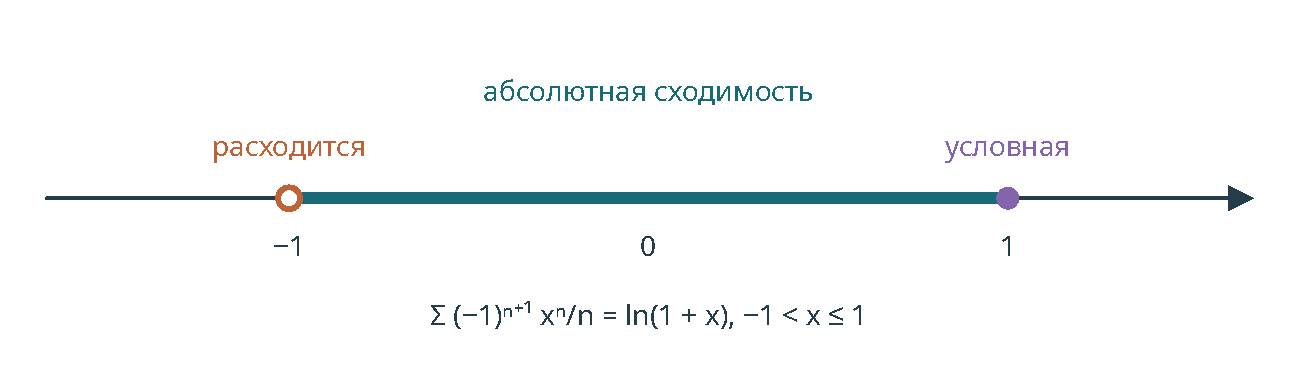
\includegraphics[width=0.95\linewidth]{figures/log-interval.pdf}
\captionof{figure}{Для ряда логарифма: расходимость при −1, абсолютная сходимость внутри и условная при 1.}\label{fig-log-interval}
\end{minipage}
\end{center}

\subsection{Биномиальный ряд}\label{sec-power-series-05-4}

\begin{equation}
(1+x)^p=\sum_{n=0}^\infty\binom pn x^n,
\qquad\binom p0=1,\quad
\binom pn=\frac{p(p-1)\cdots(p-n+1)}{n!}\ (n\ge1).
\label{eq-binomial-series}
\end{equation}

Для \(p\in\mathbb R\setminus\{0,1,2,\ldots\}\) радиус равен \(1\), поскольку \[
\left|\frac{c_{n+1}}{c_n}\right|=\left|\frac{p-n}{n+1}\right|\longrightarrow1.
\] Равенство выполняется при \(|x|<1\); сходимость в концах требует отдельного исследования.

Если \(p\) --- неотрицательное целое число, ряд обрывается и является многочленом; тогда \(R=+\infty\). Для \(n=0\) произведение в числителе пустое и равно единице.

На вещественных отрезках разложения экспоненты, синуса и косинуса следуют из формулы Тейлора и оценки остатка; комплексные формулы задают их стандартные целые продолжения. Для логарифма можно проинтегрировать геометрический ряд \(1/(1+x)=\sum_{n\ge0}(-x)^n\) на отрезке внутри \((-1,1)\). Для биномиального ряда коэффициенты удовлетворяют \((n+1)c_{n+1}=(p-n)c_n\). Поэтому его сумма \(B\) решает \((1+x)B'=pB\), \(B(0)=1\); на \((-1,1)\) отсюда \(B=(1+x)^p\).
